% Format adapted from archive/legacy/docs/geccoPaper/main.tex; historical text untouched.
\ifdefined\namedversion
\documentclass[sigconf,dvipsnames]{acmart}
\else
\documentclass[sigconf,dvipsnames,anonymous,review]{acmart}
\fi
\setcopyright{none}
\settopmatter{printacmref=false}
\acmDOI{}
\acmISBN{}
\acmConference[ManiGuard pilot]{ManiGuard pilot in GECCO format}{19 October 2026}{}
\usepackage{xurl}
\setlength{\emergencystretch}{3em}
\graphicspath{{../../figures/ManiGuard/phase3-part1/}{../../figures/ManiGuard/phase3-followup/}{../../figures/ManiGuard/phase3-part4/}}
\begin{document}
\title{An Evolutionary Safety Dial for Frozen Manipulation Policies: A Physically Audited Pilot}
\subtitle{Execution pilots, forecast audit and counterexample premise, 19 October 2026}
\author{Sachin Mohan}
\affiliation{\institution{University of the Witwatersrand}\city{Johannesburg}\country{South Africa}}
\email{2699183@students.wits.ac.za}
\renewcommand{\shortauthors}{Mohan}
\begin{abstract}
Can a compact execution controller improve safe completion around a frozen
manipulation policy? In ManiGuard Clutter, Part 1 allocates 24 simulator episodes
to evolutionary search and 24 fresh episodes to one frozen finalist at three dial
strengths. Its training lead does not persist: identity safely completes 5/8 episodes
with no observed violation, versus 3/8 with two violations at half strength and 4/8
with two violations at full strength. Part 2 separates query timing from restraint
in sixteen new episodes. Identity, fixed-eight and correction-triggered execution
each safely complete 3/4, versus 2/4 for fixed-four, with one violation per condition.
The adaptive trigger never refreshes early; fixed-four more than doubles query
cost without improving measured safe completion. Part 3 prospectively tests a
frozen visual dynamics ensemble before allowing a matched evolutionary allocation;
its forecast audit fails accuracy despite adequate event support, gating the
physical optimizer comparison. Four-action error is 45.1\% worse than persistence,
and correction calibration collapses to ordinary disagreement trust. Part 4 then
tests a direct uprightness-event predictor on 24 verified historical trajectories.
Its development operating point alarms on 2,045/2,229 negative windows, with no
confident miss among one first-event episode; its frozen gate stops physical
counterexample acquisition before new simulator interaction. We preserve
causal executed-action histories, native outcomes, videos and continuous allocation
accounting. These descriptive pilots establish neither optimizer superiority nor
calibrated physical risk.
\end{abstract}
\begin{CCSXML}
<ccs2012><concept><concept_id>10010147</concept_id>
<concept_desc>Computing methodologies</concept_desc>
<concept_significance>500</concept_significance></concept></ccs2012>
\end{CCSXML}
\ccsdesc[500]{Computing methodologies}
\keywords{evolutionary search, execution adaptation, manipulation, safety, frozen policies}
\maketitle

\section{Question and scope}
Task completion can conceal a manipulation policy's physical specification
violations. ManiGuard separates task success from safety using runtime monitors
over physics-grounded predicates~\cite{maniguard}. We test whether a small execution
controller can improve safe completion around a frozen Clutter policy, and whether
an external dial exposes a useful measured trade-off. All physical outcomes here
are measured in simulation. The monitor labels actions' consequences; it does not
filter commands.

Part 1 implements its plan at planning commit \texttt{8df7ac9}. The
machine-readable protocol was frozen before search. It contains the controller
domain, information restrictions, source hashes, scene partitions, schedules,
selection rules and absolute deadlines. The work establishes an executable and
auditable experiment. It provides no optimizer-superiority or safety-guarantee claim.

\section{Part 1: controller and frozen protocol}
The genome has four categorical coordinates: free-motion joint-target cap
$\{\varnothing,.12,.08,.04\}$ rad, grasp cap
$\{\varnothing,.08,.04,.02\}$ rad, smoothing $\{1,.75,.5\}$, and query horizon
$\{4,8,16\}$. This defines 144 points. The neutral genome disables caps and uses
smoothing one and horizon eight.

For proposed arm targets $p$, measured joints $q$ and smoothing $\alpha$, define
$r=q$ on the first action and the previous actual environment input thereafter.
The anchor computes
\begin{equation}
 z=r+\alpha(p-r),\qquad
 a=q+\operatorname{clip}(z-q,-c,c),
\end{equation}
with $a=z$ when the applicable cap is disabled. The fixed causal finger heuristic
selects the grasp cap: absolute finger positions are in $[.003,.035]$, their
maximum change is below $.002$, and the proposal closes the gripper. It does not
identify the held object.

The episode-constant external dial $d$ applies $p+d(a-p)$ to the arm and uses
\begin{equation}
 h(d)=\left\lfloor8+d(h_\theta-8)+.5\right\rfloor.
\end{equation}
Zero bypasses arithmetic exactly; one returns the anchor directly. Native gripper
binarization, downstream clipping and termination remain intact. History updates
from the final clipped environment input, before low-level actuator processing.
The controller uses only proposals, measured arm/finger positions and that causal
history. Object states, goal labels and monitor predicates are excluded. Caps
bound target displacement rather than force or collision probability.

Search runs only at $d=1$, using PCG64 seed 20261018. Population zero contains
identity and three distinct uniform random points. Each of three populations has
four slots, evaluated on two training assignments. The next population copies
the best point for fresh physical re-evaluation and creates three mutated children
from the best two parents. The declared categorical mutation kernel rejects
unchanged children and within-population duplicates; stable birth order resolves
ties, with the copied elite first. Fitness is
\begin{equation}
 \overline U=\operatorname{mean}\bigl[\mathbf1(S_{\rm req})-2\mathbf1(V)\bigr],
\end{equation}
where $V$ is raw \texttt{ltl\_violated}, $C_{\rm req}$ combines native success with
the pinned Clutter checklist, and $S_{\rm req}=C_{\rm req}\land\neg V$.
Infrastructure failures have no fitness. Only the final evaluated population can
supply the finalist.

Engineering uses \texttt{task\_0040/base}; search uses tasks 0034 and 0002; comparison
uses tasks 0029 and 0032. Whole-task partitions are preserved and test scenes remain
untouched. Training base seeds are $1000+10g+i$; comparison uses $2000+10j+r$ with
four repetitions per scene. The native evaluator derives sampling seeds as CRC32
of the base seed and scene, masked to 31 bits. The server resets a stream for each
episode ID. Independent schedule seed 20261019 seals adjacent three-dial blocks,
cycling all six permutations before repetition. Scenes are conservatively treated
as exposed; the comparison tests fresh repetitions.

\begin{figure*}[t]
\centering
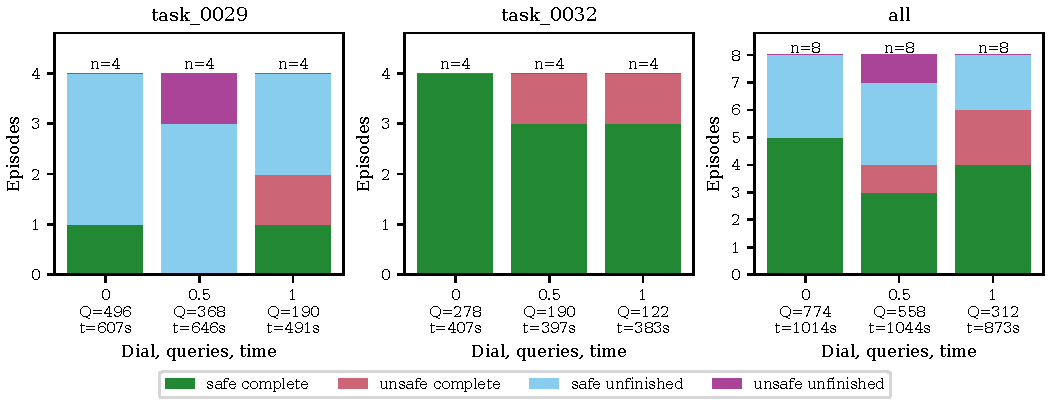
\includegraphics[width=\textwidth]{paper-outcomes.pdf}
\caption{Every fresh outcome, per scene and pooled. Each scene has four episodes per
setting; pooled denominators are eight. $Q$ is policy queries and $t$ is summed outer
episode-process time. Unsafe completion remains separate from safe completion.}
\Description{Three stacked bar charts show identity with five pooled safe completions
and zero violations, midpoint with three safe completions and two violations, and
full strength with four safe completions and two violations.}
\label{fig:outcomes}
\end{figure*}

\section{Part 1: search and fresh comparison}
Population-zero timing selected the full 48-episode allocation before selection
inspected scores. The shared eight episodes count once. The planning duration was
$\max(417\text{ s},1.25\times\text{slowest})=417$ s; the remaining estimate was
16,980 s against 21,149.97 s available. The predefined 28-episode fallback was unused.
All full jobs retain the native 1,100-action horizon and native early success.

\begin{table}[t]
\caption{Every population's mean candidate utilities, in birth order. The elite is
physically re-evaluated rather than retaining historical fitness.}
\label{tab:search}
\begin{tabular}{clcc}
\toprule
Population & Utilities & Safe complete & Violating \\
\midrule
0 & .5, 1, .5, 1 & 6/8 & 0/8 \\
1 & 1, 1, 0, .5 & 5/8 & 0/8 \\
2 & .5, 1, .5, $-.5$ & 5/8 & 1/8 \\
\bottomrule
\end{tabular}
\end{table}

The selected genome is $[3,3,0,2]$: free cap .04 rad, grasp cap .02 rad, smoothing
one, horizon sixteen. It is a new offspring of population one's second eligible
parent. It safely completes both final training episodes. The copied elite scores
only .5 in its last re-evaluation (Table~\ref{tab:search}, Figure~\ref{fig:lineage}).
One discarded search candidate completes unsafely; its outcome and costs remain.
The finalist's file hash is sealed before comparison, and all three settings use it.

\begin{figure}[t]
\centering
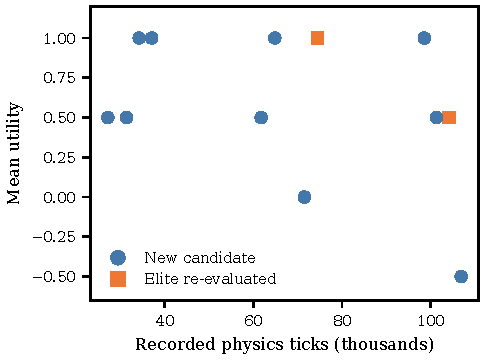
\includegraphics[width=\linewidth]{paper-lineage.pdf}
\caption{All twelve candidate measurements versus cumulative recorded physics ticks,
including engineering and the failed check. Squares distinguish re-evaluated elites.
These mixed-candidate measurements are not a single policy's estimated rate.}
\Description{Candidate mean utilities range from minus one half to one. The retained
elite falls from one to one half on its final fresh seed pair.}
\label{fig:lineage}
\end{figure}

Fresh safe completion is 5/8 at identity, 3/8 at midpoint and 4/8 at full strength
(Figure~\ref{fig:outcomes}). Full minus identity is $-1/8$, or $-12.5$ percentage
points, with two additional violating episodes. Full strength achieves six total
requested completions, but two are unsafe. Benchmark success and requested
completion agree on all 24 comparison episodes, with separate labels preserved.
No setting is selected or tuned against these outcomes.

On task 0029, safe completions are 1/4, 0/4 and 1/4. On task 0032, they are 4/4,
3/4 and 3/4. Each adapted setting records one violation on each scene. The first
failing predicate is \texttt{container\_upright=false} on task 0029 and
\texttt{obstacles\_upright=false} on task 0032. Both full-strength violating episodes
later reach the goal. The three-point response supports no calibrated or monotonic
physical-risk interpretation (Figure~\ref{fig:dial}).

\begin{figure}[t]
\centering
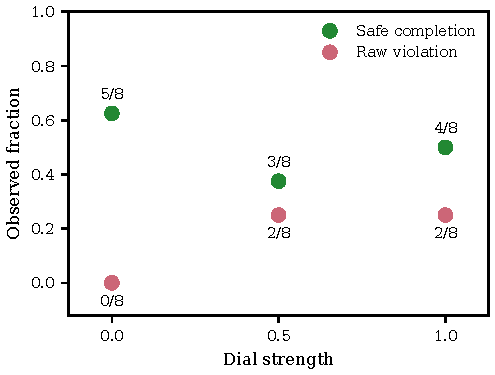
\includegraphics[width=\linewidth]{paper-dial-response.pdf}
\caption{Measured safe-completion and violation fractions with explicit denominators.
Points are descriptive; no continuous risk curve is fitted.}
\Description{Safe-completion fractions are five eighths, three eighths and four
eighths; raw violation fractions are zero, two eighths and two eighths.}
\label{fig:dial}
\end{figure}

\begin{table}[t]
\caption{Fresh interaction and process costs. Changed commands compare exact
numerical inputs; cap activation is reported separately in the audit.}
\label{tab:cost}
\begin{tabular}{crrrr}
\toprule
Dial & Actions & Queries & Process (s) & Changed \\
\midrule
0 & 6,160 & 774 & 1,014.0 & 0.00\% \\
.5 & 6,656 & 558 & 1,043.6 & 4.51\% \\
1 & 4,928 & 312 & 873.5 & 8.36\% \\
\bottomrule
\end{tabular}
\end{table}

Query latency totals are 76.8, 55.2 and 31.3 s respectively. Lower query cost at full
strength accompanies worse measured safety and safe completion; changing commands
and query horizon together prevents a mechanism-specific causal claim.
Contact/grasp episode counts, each out of eight, are $(5,5)$, $(5,4)$ and $(7,6)$.
The grasp heuristic activates on 955 midpoint and 1,325 full-strength actions; anchor
caps activate on 235 and 350. Identity's diagnostic anchor counters do not change
commands. Non-engagement in several unfinished episodes limits interpretation of
zero violations alone.

\begin{figure}[t]
\centering
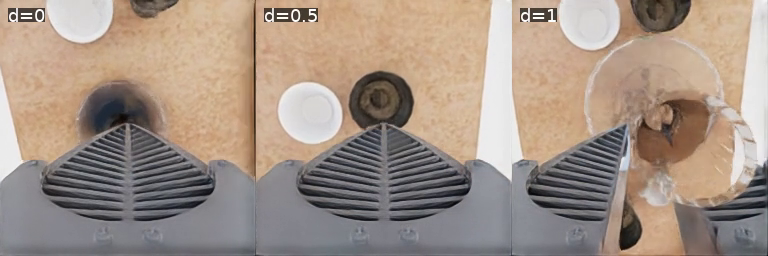
\includegraphics[width=\linewidth]{frames/task_0029-base-seed2000-wrist-t18s.png}\par
\smallskip
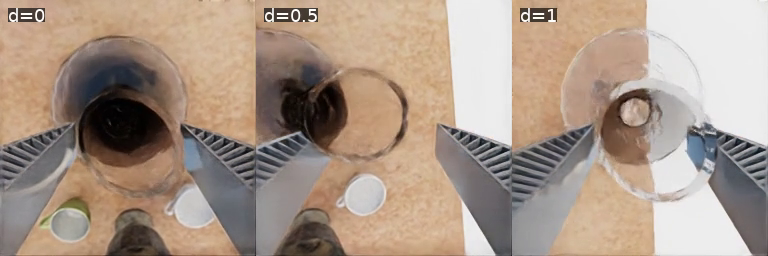
\includegraphics[width=\linewidth]{frames/task_0029-base-seed2002-wrist-t18s.png}\par
\smallskip
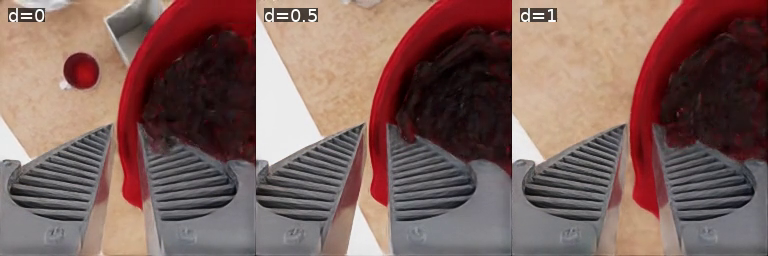
\includegraphics[width=\linewidth]{frames/task_0032-base-seed2013-wrist-t18s.png}
\caption{Actual wrist-video frames at 18 s; columns are dial 0, .5 and 1. Top:
seed 2000, where full strength later safely completes while the other settings time
out. Middle: seed 2002, where midpoint and full strength lose container uprightness;
full strength later completes unsafely. Bottom: seed 2013, where full strength loses
an obstacle's uprightness before its unsafe completion. These illustrations were
selected after outcomes. All sixteen fixed-time camera strips and all sixteen
complete three-setting videos are saved, covering every block. No physics is replayed.}
\Description{Three matched wrist-image strips show the same scene and nominal time
under the three dial settings, including the initially promising and adverse cases.}
\label{fig:frames}
\end{figure}

\section{Part 1: engineering and provenance}
CPU verification passes 33 Part 1 tests and 109 regression tests, with four skips.
Checks cover identity, causal clipped-action history, caps, finger switching,
interpolation, query schedules, seeded evolution, evidence corruption and owned
process-group cleanup. Three successful engineering checks use 32 actions each and
4/6/8 queries for an engineering horizon-four anchor. Chunks support horizon sixteen.
One earlier check fails after one completed query and zero policy actions because
strict JSON rejects infinite native action bounds. Logging is fixed before search,
without changing clipping. A naming bug produces nested engineering paths; these
are preserved and the coordinator is repaired before search. All 48 full episodes
pass physical trace replay and provenance audits.

\begin{table}[t]
\caption{Complete attempt accounting. Physics covers post-application callbacks;
pre-subscription advances are unknown for all 52 attempts.}
\label{tab:ledger}
\begin{tabular}{lrrrr}
\toprule
Work & Attempts & Actions & Queries & Physics ticks \\
\midrule
Engineering & 4 & 96 & 19 & 920 \\
Search & 24 & 17,318 & 1,738 & 105,972 \\
Comparison & 24 & 17,744 & 1,644 & 108,528 \\
Total & 52 & 35,158 & 3,401 & 215,420 \\
\bottomrule
\end{tabular}
\end{table}

All 3,401 queries complete; the failed check is a logging failure. There are 35,678
environment-step attempts and returns, 1,795.17 recorded simulated seconds, 360.03 s
of query latency and 5,982.17 s of outer episode-process time. Counts include all
initialization, discarded candidates and copied elites. Pre-subscription physics
is unknown, not zero; failed-attempt counters remain lower bounds. Overlapping
server durations do not add allocated GPU-hours.

The user-confirmed replacement is Vast instance 56582094 with one RTX 4090 and driver
575.57.08, verified through the kernel, \texttt{nvidia-smi} and provider. The originally
requested 56578764 identity is retained as provenance. No host driver is changed.
Five-second memory samples reach 17,714 MiB (17.3 GiB), without bounding unobserved
peaks. CPU/memory quotas are 30.6 cores and approximately 299 GiB.

Separate uv-managed Python 3.10 simulation and Python 3.11 policy environments use the
pinned ManiGuard, BEHAVIOR and openpi stack~\cite{openpi}. The checked legacy renderer
supplies $256\times256$ RGB overview/wrist inputs with action/render/physics rates
20/20/120 Hz, raw joint control and assisted grasping. The root environment and
UNISafe installers are not used. Clutter checkpoint revision
\texttt{f572e33bdb49} (full revision in the controller export), step 7100, keeps native inference
settings. Controller exports retain all eighteen checkpoint-file hashes and code pins.

The original allocation clock starts at 16:00:37 UTC, including setup, implementation,
failed and idle work before and after replacement. During Part 1, an independent supervised guard preserves the original
23:00:37 UTC physical target and 00:00:37 UTC next-day hard end across restarts. The policy stops at 18:25:29 UTC; process/GPU checks confirm complete exit
by 18:25:57 UTC, at 2.422 allocated GPU-hours. Subsequent paper preparation, backup
and idle rental continue to count. The public audit records the later accounting
cutoff and rental-stop scope.

The evidence contains 104 native video files, including the failed check, and sixteen
matched composites covering both cameras in all eight comparison blocks. CPU
composition preserves frame order and marks ended episodes with black frames.
A 52-row public ledger, lineage, fixed-time picture gallery, frozen protocol and
controller, and all figure data accompany this note. Credential-scanned raw evidence
is preserved in the approved private dataset, with asset bundles, checkpoints and
keys excluded. The \href{https://huggingface.co/datasets/Sachioster/safety-dial-phase3-part1-20261018/tree/17dbdcb7e29a71c763f6441ac4aa8d0c7fcf6647/matched-videos}{matched-video gallery}
requires the owner's access. Git contains derived reporting artifacts rather than
raw run directories.

\section{Part 1: interpretation}
The training lead disappears in the fresh check. The controller increases observed
violations and does not improve safe completion. It is a working interface with an
adverse pilot result. Matching seeds does not equate observations: all sixteen initial
state comparisons are numerically identical, but every camera-image comparison
differs. Two exposed scenes, eight repetitions per setting and one optimizer seed
support only a descriptive conclusion. Identity's zero violations would give the
approximate 95\% upper bound $3/8=37.5\%$ even under independent homogeneous sampling;
repeated scenes further limit interpretation.

These findings motivate isolating query scheduling from caps before increasing
evolutionary search. Ordinary policy learning remains necessary for the broader
research claim. Part 1 contains no such comparison or outcome-dependent extra episode.
Parts 2 and 3 follow separately frozen plans at planning baseline \texttt{d4b8182}.

\section{Part 2: isolate correction and feedback}
Part 1 changes restraint and query horizon together. Its failure investigation
found some corrected commands followed by cached proposals, motivating a bounded
mechanism test rather than an established diagnosis. Four conditions use the same
frozen VLA: A preserves its commands and queries every eight actions; B applies the
finalist's .04/.02 rad caps at interval eight; C uses those caps at interval four;
D uses those caps with correction-triggered refresh between four and eight. The
finger heuristic, componentwise mapping and smoothing one are common to B/C/D.
There is no new evolutionary search or three-setting dial sweep in Part 2.

After actual environment input $u_t$, D accumulates
\begin{equation}
 D_k=\sum_{t\text{ since query}}
 \frac{\|p_t^{\rm arm}-u_t^{\rm arm}\|_2}{\sqrt7\,(.04\text{ rad})}.
\end{equation}
Per-coordinate differences no larger than $10^{-6}$ rad are zeroed first. The
accumulator resets on a query, preserving previous actual input and finger history.
Goal termination takes precedence; otherwise refresh occurs once $k\ge4$ and
$D_k\ge.5$, or at $k=8$. Both the correction and trigger use already executed
inputs after downstream action-space clipping. Command departure measures neither
actual displacement nor physical risk. No privileged held label, object pose or
monitor verdict enters this controller.

The frozen allocation has sixteen full episodes: tasks 0039/0010 each receive two
fresh base seeds (4000/4001 and 4010/4011), with four conditions in each matched block.
The prospective order is ABCD, BCDA, CDAB, DABC. Native horizon, goals, monitor and
policy inference remain unchanged. Engineering checks A/C/D at 32 actions each;
one pre-application import failure and two coordinator/tooling failures are retained.
There are no full-episode retries or outcome-dependent additions.

\subsection{Part 2 measured outcomes}
All sixteen full episodes pass independent action/monitor replay, source/checkpoint
and native sampling-seed checks. Safe completion is 3/4 for A, B and D and 2/4 for C;
each condition has one violating episode (Figure~\ref{fig:part2-outcomes}). Requested
completion is 3/4 in every condition. A/B/D each have one unsafe unfinished episode;
C has one unsafe completion and one safe unfinished episode. All conditions safely
complete both task 0010 episodes. On task 0039, A/B/D each safely complete one of two,
whereas C safely completes neither. These small descriptive counts support no claim
that one schedule is superior or that frequent feedback itself causes harm.

\begin{figure*}[t]
\centering
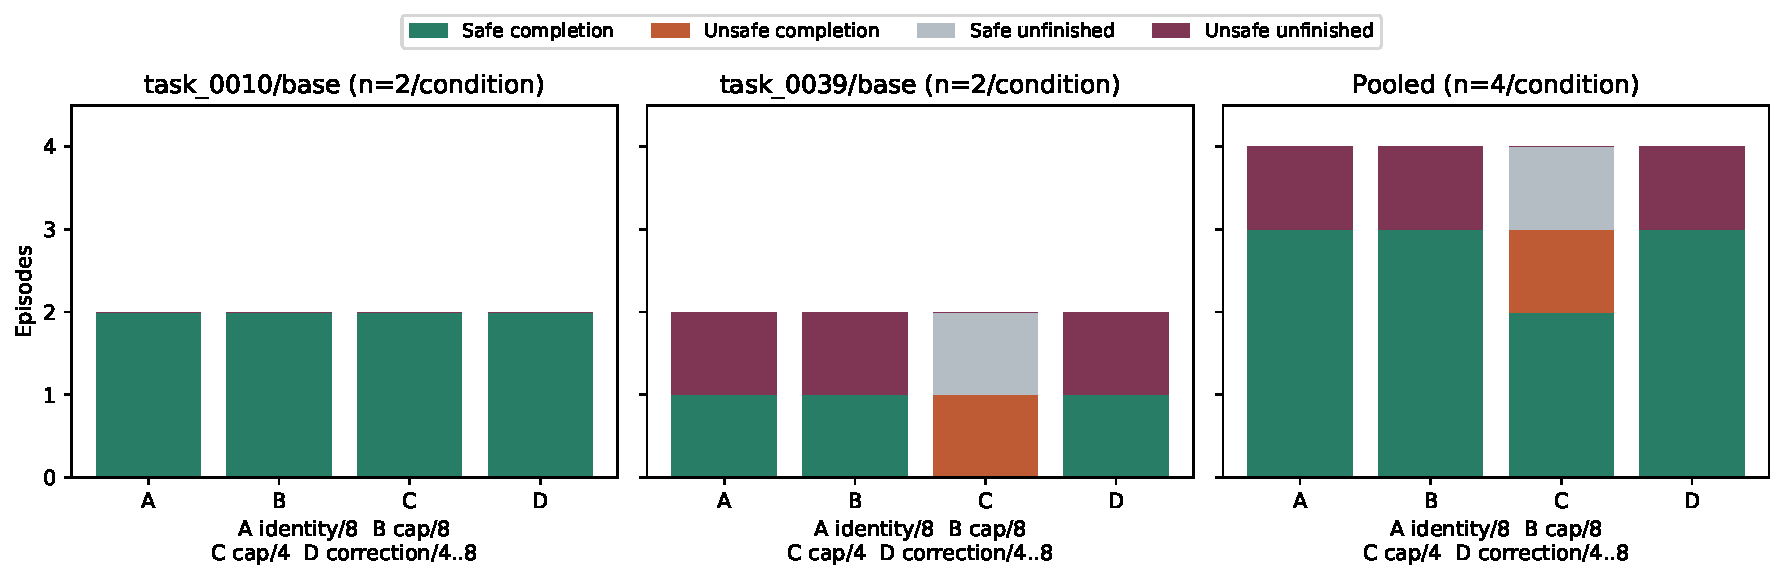
\includegraphics[width=\textwidth]{part2-outcomes.pdf}
\caption{Part 2's complete sixteen-episode sample, with unsafe completion and both
unfinished categories preserved. Each scene has two episodes per condition; pooled
denominators are four. A is identity/8, B is cap/8, C is cap/4 and D is correction/4--8.}
\Description{Pooled safe completions are three, three, two and three of four.
Every condition has one violating episode; only C completes unsafely.}
\label{fig:part2-outcomes}
\end{figure*}

The adaptive rule never changes the query schedule: every one of D's 337 actual
inter-query intervals is eight actions (Figure~\ref{fig:part2-feedback}). Its correction
threshold is crossed once, at action eight, when a query is already due. There is no
crossing at actions four through seven. Its largest accumulated correction is .60146.
Thus this run supplies no adaptive-feedback gain while leaving an actively triggering
rule untested. The threshold is retained rather than adjusted against these outcomes.
C uses 750 queries versus B's 336 without improving measured safe completion.

\begin{figure*}[t]
\centering
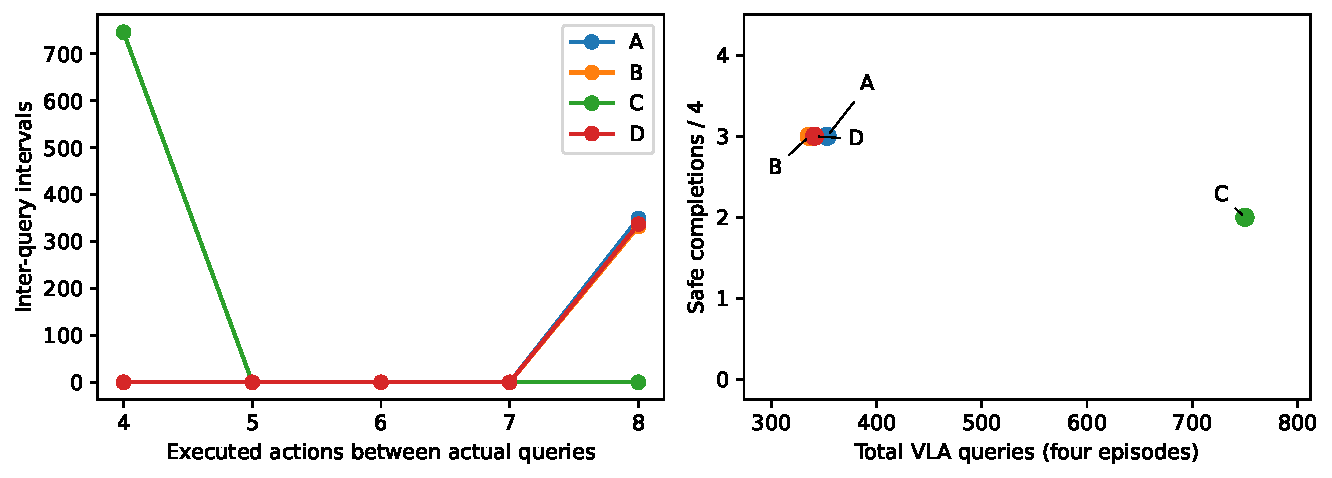
\includegraphics[width=.85\textwidth]{part2-feedback.pdf}
\caption{Observed inter-query intervals and query cost in Part 2. A/B/D always wait
eight actions; C always waits four. Safe completions have denominator four.}
\Description{The adaptive controller D shares the fixed-eight schedule, while fixed
four more than doubles queries without increasing safe completions.}
\label{fig:part2-feedback}
\end{figure*}

\begin{table}[t]
\caption{Part 2 costs. Time is measured inside each evaluator, including capture;
outer process time over all sixteen episodes is 1,897.69 s.}
\label{tab:part2-costs}
\begin{tabular}{lrrrr}
\toprule
Condition & Actions & Queries & Time (s) & Corrections \\
\midrule
A & 2,810 & 353 & 455.13 & 0 \\
B & 2,674 & 336 & 438.27 & 76 \\
C & 2,992 & 750 & 499.49 & 55 \\
D & 2,714 & 341 & 451.85 & 54 \\
\bottomrule
\end{tabular}
\end{table}

Table~\ref{tab:part2-costs} counts substantial arm changes above $10^{-6}$ rad.
Exact changed-command counters are 0/122/95/92; the additional numerical changes
are roundoff rather than further substantial cap activations. All four episodes per
condition show contact; grasp flags occur in 4/4 for A and 3/4 for B/C/D. Such flags
do not establish successful continuation after contact.

All twelve initial robot-state comparisons against A are exactly equal, but none of
the corresponding 24 camera pairs or twelve first chunks is exactly equal. Matched
scene and sampling-seed settings therefore do not identify single-episode causal
counterfactuals. The prescribed fixed-reference selection chooses B, with mean
$U=.25$ versus C's zero; no additional setting is tuned.

The full sample records 11,190 controls, 1,780 queries and 68,516 post-subscription
physics ticks. Engineering adds 96 controls, sixteen queries and 834 known ticks;
the pre-application failure retains unknown native counters. Synthetic CPU checks
precede engineering, but recorded physical-input replay first audits engineering
jobs rather than preceding them as requested by the plan. This chronology deviation
is explicit; all engineering replay passes before the full comparison freeze.
Twenty-four targeted CPU checks pass across Parts 2 and 3. Every native camera clip,
all eight matched Part 2 videos and complete event-picture strips are preserved.


\section{Part 3: model feasibility before evolutionary use}
The proposed contribution concerns which motion mutants merit physical evaluation,
using observed errors conditional on execution correction. Dynamics-assisted
skill search already exists~\cite{daqd}; frozen visual-feature prediction and short
rollouts also have precedent~\cite{dinowm,mbpo}. These ingredients and an optimizer
substitution do not establish novelty. We test a compact feasibility stage before
spending the physical optimizer-comparison allocation.

\paragraph{Data and information.}
The Part 1 training traces lack later exact images and numerical margins; exposed
Part 1 comparison episodes are excluded. Before fitting, the declared eight-episode
recording option is sealed: B/C on tasks 0046/0006, two fresh seeds per task. All
sixteen Part 2 episodes on 0039/0010 are fitting data; four 0046 episodes calibrate;
four 0006 episodes audit. Whole tasks, seeds and trajectories remain separated.
The 0048/0050 final comparison and main-study test partition are outside development.
Acquisition is charged once, including reused common data.

Passive capture, identical across all Part 2/3 recording conditions, saves the
already extracted overview/wrist RGB at every step without rendering or advancing
physics. Evaluation-only numerical targets reproduce the native float32 local
$+Z$ tilt calculation and per-object thresholds, plus negative target-to-goal
distance. Targets never enter the live controller or dynamics input. Numerical
uprightness is audited against native Boolean bindings. The final image remains
saved but is omitted from model pairs without its missing subsequent two-finger
proposal frame. A spatial distance readout is distinct from the native held-object
goal; tilt is distinct from spill/drop safety.

\paragraph{Frozen predictive system.}
A pinned DINOv2 small encoder~\cite{dinov2} produces $2\times2$ spatially pooled
patch features from each camera, 3,072 coordinates in total. Fitting-only
standardization and randomized PCA retain 32 visual coordinates. Seven measured
arm joints and both finger positions remain separate. Five episode-bootstrap
128/128-unit residual MLPs predict the next standardized visual/robot state,
conditioned on the current and previous state and previous/current actual
8-coordinate environment inputs. Each trains for 30 epochs with fixed settings.
History shifts causally during rollouts of at most four actions. PCA is compression;
the action-conditioned residual networks supply the dynamics.

Ridge heads estimate minimum upright margin and short-term progress. The audit
compares persistence, fitted ridge, action-shuffled ridge and the same ensemble
with mispaired action sequences, changing-state windows, and actual versus
predicted future-state readouts. Raw pooled features, PCA and a same-size random
projection diagnose representation/readout limitations. Correctly paired and
shuffled sequences share the same trained ensemble in the action-dependence gate.
Pre-fitting source refinements preserve their original receipts; numerical criteria,
data groups, physical slots and model hyperparameters are unchanged.

\paragraph{Reliability and prospective search.}
M trusts ensemble disagreement; C uses an empirical conditional .8-error-quantile
lookup by factual correction, with sparse bins falling back to the unconditional
quantile and unsupported contexts abstaining. Both use nominal .5 calibration
acceptance; actual acceptance and consequential errors must also be reported.
These are empirical allocation heuristics, not calibrated safety probabilities.
Planned counterfactual correction never becomes a factual residual without execution.

If the sealed forecast criteria permit, the 64-episode physical pilot evaluates a
shared four-controller initial population on two cases (eight episodes once),
three four-slot descendant populations on two fresh cases (24), two shortlisted
controllers per method on two confirmation cases (12), and identity, one fixed
Part 2 reference and three frozen finalists on four fresh blocks (20). Each
method retains an actually re-evaluated elite, one unguided timing mutant and
two cap mutants from a common pool of at most sixteen proposals. The known
four-command prefix cannot rank later query timing, so timing genes stay in
physical exploration. Abstention removes a model recommendation rather than a
candidate's exploration eligibility. All deployed controllers share the same
information and family; actual mean $U$ determines selection and confirmation.
No learned online action veto is installed. Three additional 32-action engineering
attempts are available before eligible search, with no full-episode replacement.
The deployed family has 160 genotypes: free caps
$\{\varnothing,.12,.08,.04\}$ rad, grasp caps
$\{\varnothing,.08,.04,.02\}$ rad, thresholds $\{0,.5,1,2,\varnothing\}$,
and minimum intervals $\{4,6\}$, with maximum eight and smoothing one fixed.


\subsection{Part 3 forecast audit and scientific gate}
The eight common recordings and all model workers complete normally. The forecast
audit fails accuracy, with every support requirement satisfied; the physical
64-episode optimizer comparison is therefore unstarted by protocol. No Part 3
finalist, lineage, optimizer outcome or superiority result is asserted. This is a
measured negative feasibility result, not a time-limited incomplete stage.

The corpus has sixteen fitting, four calibration and four audit episodes. Audit
contains 552 four-action query-start windows, of which 263 exceed the fitting
median displacement, 101 are near the upright boundary and 99 end with negative
margin. Near-boundary events occur in four calibration and two audit episodes,
with one audit episode crossing the boundary. There are 152 varying-progress
windows. Windows are correlated within four episodes on one held-out task; they
are not 552 independent safety trials.

On changing windows, one-action error is .2962 for the ensemble versus .2318 for
persistence. Four-action errors are .4120 for persistence, .5179 for ridge, .5214
for action-shuffled fitted ridge, .6145 for the same ensemble with shuffled action
prefixes and .5979 for correctly paired actions (Figure~\ref{fig:part3-forecast}).
The ensemble is 27.8\% and 45.1\% worse than persistence at one and four actions.
Its 2.69\% improvement over mispaired actions passes the action-dependence check,
but does not compensate for absolute/reference failures (Table~\ref{tab:forecast}).
The actual-state head also fails before dynamics prediction is introduced.

\begin{figure*}[t]
\centering
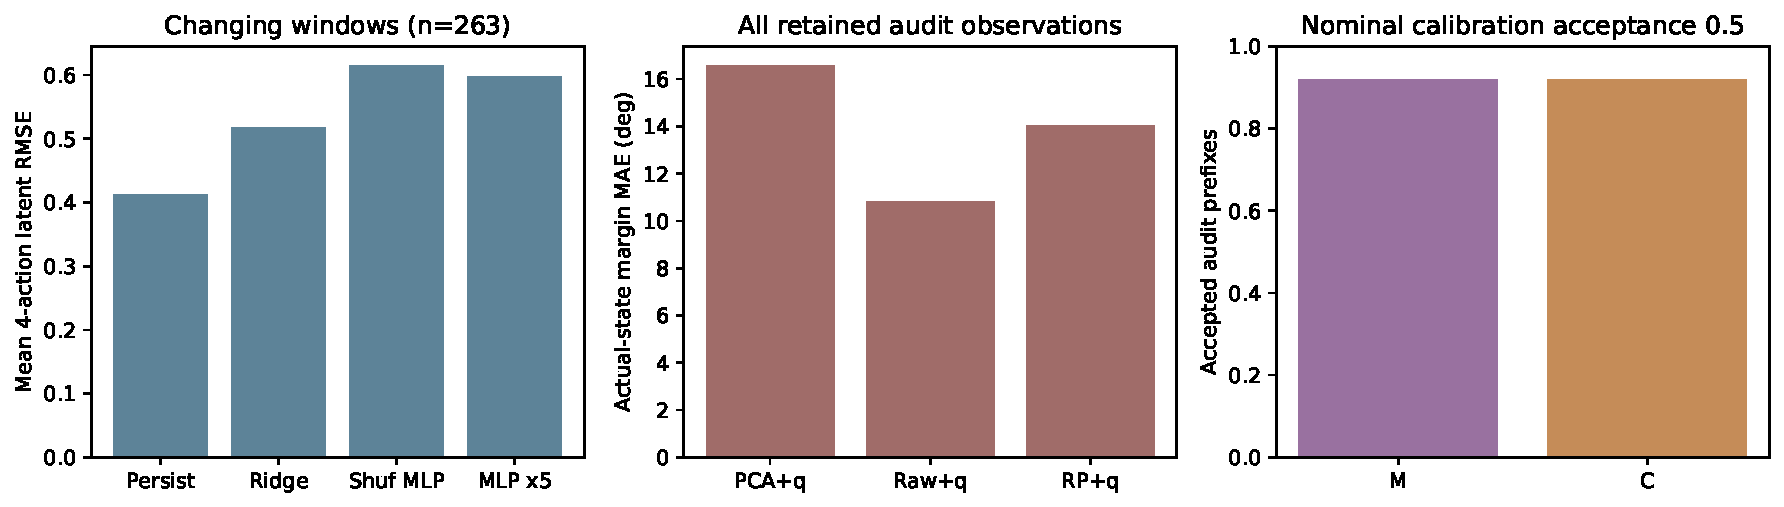
\includegraphics[width=\textwidth]{part3-forecast.pdf}
\caption{Part 3 forecast audit. Left: mean per-window standardized visual-latent RMSE
on 263 changing windows. The shuffled-prefix control uses the same ensemble.
Middle: actual-state readouts on every retained audit observation, with robot state
included. Right: actual acceptance over all 552 audit prefixes. These quantities
are not safety probabilities.}
\Description{The ensemble is worse than persistence and ridge. Raw features improve
the combined readout relative to PCA, while both trust methods accept about 92 percent.}
\label{fig:part3-forecast}
\end{figure*}

\begin{table}[t]
\caption{Frozen forecast criteria and observed values. All event-support criteria
pass; seven accuracy/usefulness criteria fail. Degrees and millimetres are physical
readout errors; latent errors use standardized coordinates.}
\label{tab:forecast}
\begin{tabular}{lrr}
\toprule
Criterion & Measured & Required \\
\midrule
One-step improvement & $-27.8\%$ & $\ge5\%$ \\
Four-step improvement & $-45.1\%$ & $\ge5\%$ \\
Shuffled-prefix improvement & $2.69\%$ & $\ge2\%$ \\
Ensemble/ridge error & 1.155 & $\le1.05$ \\
Actual-state margin MAE & $16.17^\circ$ & $\le10^\circ$ \\
Near-boundary forecast MAE & $18.56^\circ$ & $\le10^\circ$ \\
Progress MAE & 79.01 mm & $\le30$ mm \\
Progress ranking, Spearman & .126 & $\ge.25$ \\
False reassurance & 0/99 & $\le.10$ \\
M/C actual acceptance & 507/552 & $\ge.10$ \\
Sixteen-candidate screening & .810 s & $\le30$ s \\
\bottomrule
\end{tabular}
\end{table}

All 818 calibration prefixes fall below the first .5 correction boundary, with
maximum .17839. Sparse-bin fallback makes every conditional error quantile equal
to .80913. C is then a positive affine transform of M; the same support conditions
and transformed median thresholds produce exactly equal audit acceptance masks:
507/552 each, or 91.85\%, versus 50\% on calibration (Figure~\ref{fig:calibration}).
Audit bins contain 551/1/0/0/0/0 prefixes. This calibration supplies no distinct
correction-dependent allocation rule. It is retained rather than repaired using
held-out outcomes. Zero false reassurance among 99 correlated negative-margin
windows from one episode does not validate a safety guarantee.

\begin{figure*}[t]
\centering
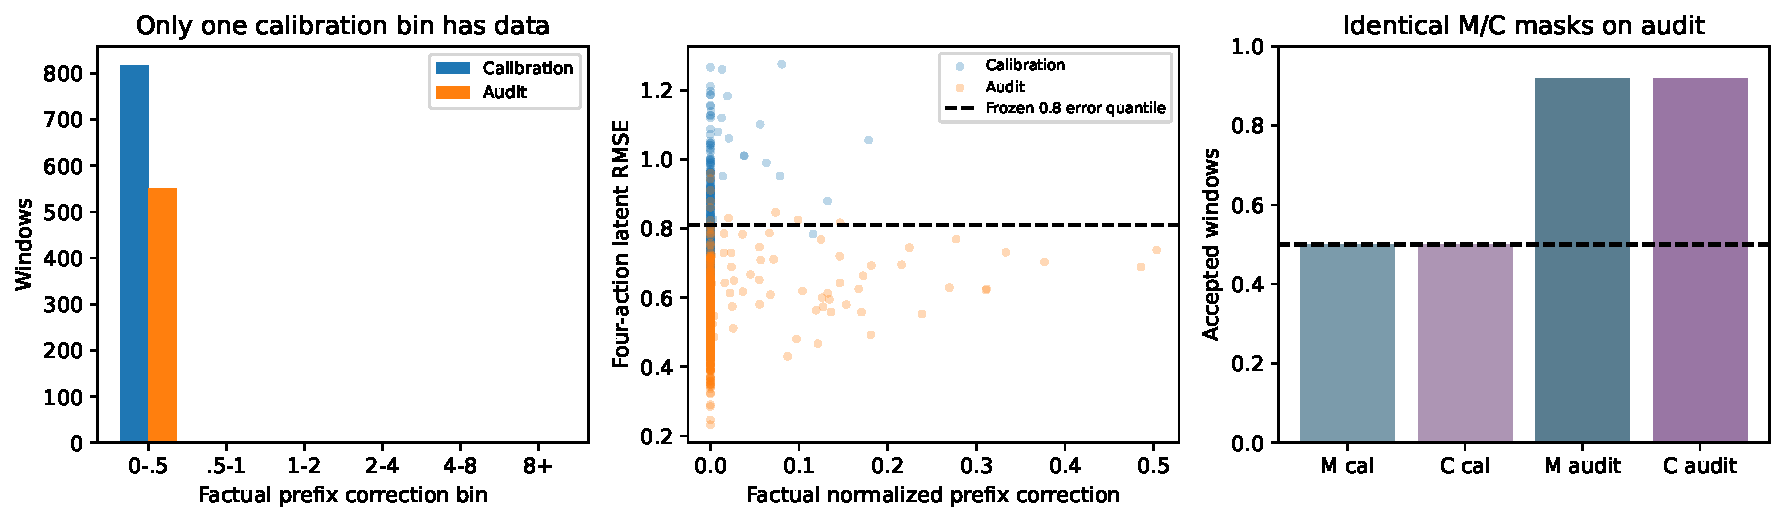
\includegraphics[width=\textwidth]{part3-calibration.pdf}
\caption{The frozen correction calibration collapses to one populated bin. Empty
bins use the unconditional .8-error quantile. M and C have equal acceptance masks,
and their nominal calibration acceptance does not persist on the audit task. No
additional episode or changed threshold follows this result.}
\Description{All calibration data occupy the first correction bin. The constant
error lookup makes correction-dependent trust equivalent to disagreement trust.}
\label{fig:calibration}
\end{figure*}

A post hoc, frozen-weight diagnostic matches every head on the same 552 actual
future observations. Margin MAE is $16.17^\circ$ for PCA plus robot state,
$11.03^\circ$ for raw pooled features plus robot state, $12.82^\circ$ for a random
projection plus robot state, and $8.54^\circ$ for visual-only PCA. Their progress
errors are 80.57/52.94/104.53/41.13 mm. The visual-only contrast motivates testing
cross-task covariate conditioning; it prevents diagnosing PCA information loss
alone as the established cause. No head is replaced after audit. Fitting PCA
retains 82.05\% of visual variance, without certifying task/safety information.

The common recordings yield 3/8 safe completions, 4/8 violations and 5/8 unfinished
episodes, with no unsafe completion. Calibration has 0/4 completions and three
violations; audit has three safe completions and one violation. These data-acquisition
outcomes are not an evolutionary comparison. Both native cameras, eight matched
recording videos and complete event/episode picture strips are preserved.


\section{Part 4: counterexample acquisition premise}
\label{sec:part4}
Part 4 asks whether diverse physical hazards confidently missed by a small
predictor can improve held-out prediction per acquisition cost. The planned
comparison is stratified random sampling (R), uncertainty-guided mutation (U),
concentrated missed-hazard evolution (E), and diversity-preserving evolution (D).
Eight shared seeds, twelve new slots per method, eight confirmations and sixteen
common audit episodes give an 80-episode ceiling, conditional on predictor,
scene/reset and throughput feasibility. Policy and execution remain fixed; the
predictor observes execution without changing actions.

The ingredients have precedents: quality-diversity scenario
generation~\cite{fontaine2021scenarios}, uncertainty-based VLA annotation
acquisition~\cite{failurespot}, and counterexample-guided joint agent/critic
repair~\cite{boetius2024repair}. Their tasks and labels differ. No novelty or
optimizer-superiority claim follows from implementing these ingredients.

\subsection{Frozen causal target and direct predictor}
The offline protocol is pushed at \texttt{e66c2f9} before the Part 4 label audit;
the initial implementation follows at \texttt{9c9ccd9}. We restore and hash-check
the exact 24 Part 2/3 feature records and corresponding traces from private dataset
revision \texttt{f070abcb707b}. Its 3.34 GB raw archive passes SHA-256 verification.
Pinned native object scopes and tilt thresholds agree with numerical margins in
37,362 proposition-observation checks. Robot measurements, proposals, actual
environment inputs and query flags match their exact recorded trace entries.

The target is the first native uprightness violation of any protected object.
At observation $t$, predict its occurrence in the next $H=8$ actions while no
violation has yet occurred. A useful warning must occur in
$[\tau-8,\tau-4]$, where $\tau$ is first onset. At 20 Hz these specify a
0.4 s horizon and a 0.2 s deadline within the fixed-eight execution cadence.
History ends at $t$; actual executed commands stop at $t-1$. We exclude
already violated states, insufficient history and windows without eight real
future observations. There is no terminal padding or unsuccessful-episode label
substitution. One episode supplies at most one first-event warning denominator.

Fit-only PCA reduces the frozen two-camera DINOv2 features from 3,072 to 32 values.
The 255-dimensional primary input combines the current and four preceding
visual/robot observations, current proposed command, four previous actual commands,
known controller settings and query age. Controller metadata conditions the
historical A/B/C/D mixture. Privileged object states, monitor predicates, event time,
task identity, scene genes and future observations/actions are excluded.

Five episode-bootstrap MLPs each have one 64-unit tanh layer and exactly 500 Adam
updates of batch size 256. Bootstrap sampling is stratified by whole task.
Per-trajectory window contributions are capped at 256, with retained positives,
inverse-inclusion-weighted sampled negatives and equal episode mass before class
balancing. Fixed L2 logistic models provide full-input and visual-only references.
Platt probability calibration and each operating threshold use the common
calibration task. Architecture, seeds, updates, targets and thresholds are not
retuned using development outcomes. Encoder, dynamics and VLA weights stay fixed.

\begin{table}[t]
\caption{Part 4 exposed historical development data. Positive windows are
correlated within the first event; the Part 3 audit is not a fresh Part 4 audit.}
\label{tab:part4-support}
\begin{tabular}{lrrrr}
\toprule
Group & Tasks & Episodes & Events & Pos./windows \\
\midrule
Fit & 2 & 16 & 4 & 32/8,390 \\
Calibration & 1 & 4 & 3 & 24/2,584 \\
Development & 1 & 4 & 1 & 8/2,237 \\
\bottomrule
\end{tabular}
\end{table}

Fitting uses tasks 0039/0010, calibration 0046 and development 0006. All four
fitting events occur on task 0039, failing the minimum two event-task criterion.
Development has one event, failing its minimum two episode criterion
(Table~\ref{tab:part4-support}). Missing support remains inconclusive. All task
variants stay in one group, the fresh final audit is not selected or opened,
and released VLA pretraining overlap remains unknown.

\subsection{The operating point fails to generalize}
The primary alarm threshold is .02995514. Its calibration false-alarm rate is
4.9801\% when episodes receive equal weight; pooled counts are 110/2,560,
or 4.2969\%. Low risk means probability at most .1. Low disagreement means
uncalibrated member-probability standard deviation at most .00204003, the
calibration negative-window 25th percentile. Calibration of the mean and the
disagreement statistic are recorded separately.

\begin{table}[t]
\caption{Part 4 development prediction at operating points frozen on calibration.
False alarms are pooled negative windows. Every model warns on the one event;
this alone does not establish a useful trade-off.}
\label{tab:part4-warning}
\begin{tabular}{lrrr}
\toprule
Predictor & AUROC & AP & False alarms \\
\midrule
MLP ensemble & .8345 & .0121 & 2,045/2,229 \\
Full logistic & .8845 & .0165 & 948/2,229 \\
Visual logistic & .9735 & .4258 & 1,575/2,229 \\
\bottomrule
\end{tabular}
\end{table}

Primary average precision (AP) exceeds the .003576 positive-window prevalence but
fails the frozen .05 minimum. Its 91.75\% negative-window false-alarm rate exceeds
the .15 maximum (Table~\ref{tab:part4-warning}). Every development episode has a
false alarm, 4/4, as does every calibration episode, 4/4. Always-alarm also misses
zero events but alarms on all 2,229 negative windows; always-safe misses 1/1 events
without false alarms. The observed 0/1 missed timely warnings therefore cannot
validate this operating point. The visual-only reference ranks better but still
alarms on 70.66\% of negative development windows; it is not substituted after the
gate fails (Figure~\ref{fig:part4-tradeoff}).

\begin{figure*}[t]
\centering
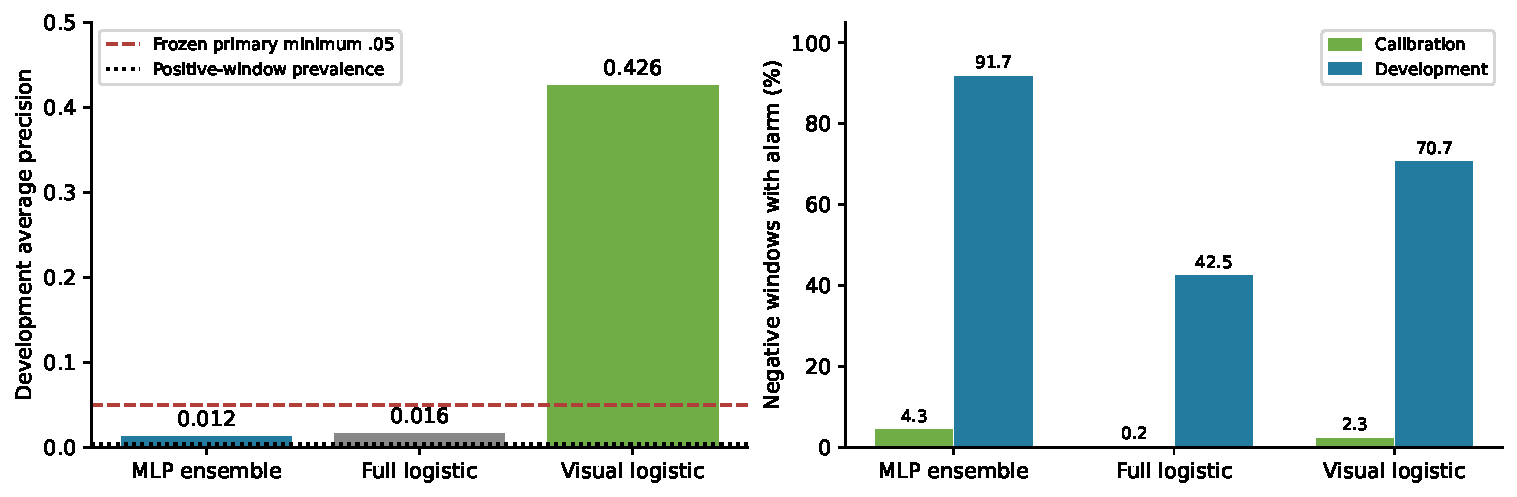
\includegraphics[width=.97\textwidth]{warning-tradeoff.pdf}
\caption{Part 4 discrimination and actual false alarms on exposed development
data. The visual-only ablation ranks the one event better, while its frozen
operating point still has excessive false alarms. Eight positive windows come
from one event, not independent failures. Calibration columns show pooled rates;
threshold selection weights episodes equally.}
\Description{Primary and full-logistic average precision are .012 and .016,
versus .426 for visual logistic. Development false alarms are 91.7, 42.5 and
70.7 percent. These rates are much higher than their calibration values.}
\label{fig:part4-tradeoff}
\end{figure*}

The primary misses 3/3 calibration events. One is a qualifying low-risk miss:
\texttt{part3-record-b0-C}, bowl\_69 onset 843, with deadline probability .0119821
and disagreement .00165808, giving descriptive quality .988018. The other two
misses have greater disagreement. The sole development event, teacup\_73 onset
307 in \texttt{part3-record-b3-B}, warns eight actions early, with deadline
probability .113333 and disagreement .196481. It is not a confident miss; all
295 negative windows in that episode alarm. The calibration case neither proves
reproducible acquisition nor supplies independent development support
(Figure~\ref{fig:part4-timelines}).

\begin{figure*}[t]
\centering
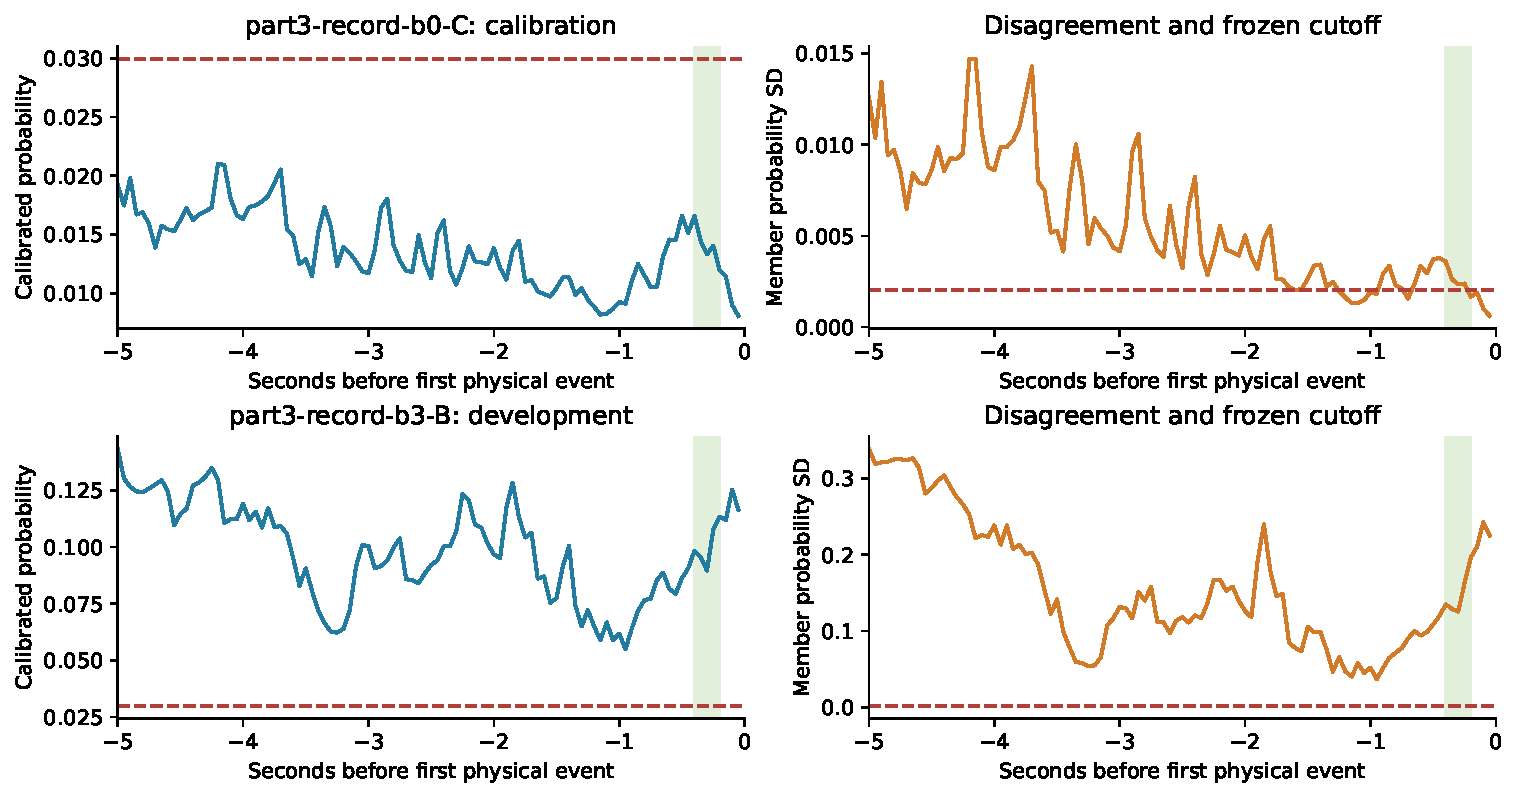
\includegraphics[width=.93\textwidth]{warning-timelines.pdf}
\caption{Historical calibration low-risk miss (top) and development event with
excessive alarms (bottom). Green marks the eligible 0.4 to 0.2 s warning interval;
red dashed lines show frozen probability and disagreement cutoffs. Scores end
before the first event. No hypothetical action branch or new physics is used.}
\Description{The calibration miss remains below the alarm threshold. Development
probabilities exceed the threshold throughout this displayed five-second prefix,
and disagreement is much larger than the low-disagreement cutoff.}
\label{fig:part4-timelines}
\end{figure*}

The frozen gate is \texttt{failed\_discrimination}, with additional support and
confident-miss failures. Shared-initial rescue requires discrimination to pass,
so those eight episodes are ineligible. Physical scene/reset engineering, all
48 acquisitions, eight confirmations, repair and sixteen audit episodes remain
unstarted. Empty stage receipts retain those distinctions; there is no generated
scene, archive elite, repaired predictor, recurrence rate or held-out repair result.
The CPU acquisition kernels and matched-update helper are implemented, with tests
for bookkeeping and information isolation, but have no physical validation here.

\subsection{Costs and preservation}
Part 4 adds zero simulator attempts, controls, physics steps, VLA queries or encoder
calls. The 24 reused donors retain their original 18,657 controls, 3,165 queries and
114,006 known post-subscription physics ticks, charged once. Their physical outcomes
are 14 safe completions, one unsafe completion, two safe unfinished and seven
violating unfinished episodes. Pre-subscription physics remains unknown; the
uprightness prediction target does not replace the other native physical outcomes.
Uprightness violations occur in 4/16 fitting, 3/4 calibration and 1/4 development
episodes. Spill occurs in 3/4 calibration episodes; no donor has a native drop
violation. Types can overlap. Task-specific proposition names are resolved from
their pinned definitions and the resulting violation flag matches every audit.

New fitting uses 2,500 MLP updates and 640,000 sampled windows. Scoring evaluates
66,055 ensemble-member windows and 26,422 reference windows. One worker fails after
training when reloading a partially reconstructed PCA estimator. Prediction resumes
from identical hash-verified weights using the explicit saved affine transform;
no second fit or model search occurs. The failed attempt and time are retained.

The existing replacement allocation is single-RTX-3090 instance 56676451, beginning
19 October 05:28:29.253 UTC, rather than the proposed 4090/5090. The physical cutoff
is 12:28:29.253 UTC and hard stop 13:28:29.253 UTC. All preparation, implementation,
reporting and idle time count from the original provider start, with an independent
supervisor-managed deadline guard. This preparation base is not a validated ManiGuard
stack, and no simulation-throughput or reset-repeatability claim is made.

Eight two-camera event strips and two 101-frame, 20 Hz videos use individually
hash-checked historical RGB. They show warning start, deadline, native onset and
post-onset observations without replaying physics. Own weights and evidence are
separately private, revision-pinned and download/hash verified; full identifiers
are in the Part 4 export and gallery linked from the paper README. Final
preservation and provider state are recorded separately from scientific termination.
This bounded result supplies no evolutionary acquisition or repair-efficacy claim.


\section{Cumulative accounting and preservation}
Parts 2 and 3 reach their accurately reported terminal outcomes. The
complete allocation contains eighty physical attempts: Part 1's 52 once,
Part 2's twenty including engineering, and eight common Part 3 recordings
(Table~\ref{tab:cumulative}). The sixteen Part 2 fitting episodes are reused rather
than recharged as new model interactions. The conditional 64-episode search and
its three engineering checks remain unstarted. Known totals are 53,911 controls,
6,582 VLA queries and 330,260 post-subscription physics ticks. One pre-application
followup failure has unknown native counters; all pre-subscription initialization
physics remains unknown. These totals are recorded lower bounds rather than zeros
for missing counters. An interim prose total of twenty Part 2 engineering queries
is corrected to the audited $4+8+4=16$; raw records and outcomes are unchanged.

\begin{table}[t]
\caption{All physical attempts, including prior experience once. The total is the
sum of known counters; one pre-application followup failure has unknown counters.}
\label{tab:cumulative}
\begin{tabular}{lrrrr}
\toprule
Stage & Attempts & Controls & Queries & Ticks \\
\midrule
Part 1, all & 52 & 35,158 & 3,401 & 215,420 \\
Part 2, engineering & 4 & 96 & 16 & 834 \\
Part 2, comparison & 16 & 11,190 & 1,780 & 68,516 \\
Part 3, recording & 8 & 7,467 & 1,385 & 45,490 \\
Part 4, offline only & 0 & 0 & 0 & 0 \\
Total & 80 & 53,911 & 6,582 & 330,260 \\
\bottomrule
\end{tabular}
\end{table}

Scientific feature extraction encodes 37,314 images in 594 calls in 127.03 s.
Training uses 11,158 transitions, 6,600 optimizer steps and 1,668,720 member examples,
taking 16.40 s. Calibration, audit and candidate-screening use 380 member calls over
48,680 examples. Synthetic CPU engineering adds 720 member calls and 22,440 examples,
1,520 training examples and ten optimizer steps, plus a two-image encoder check;
it is not empirical prediction evidence. The post hoc matched readouts add four
matrix calls over 2,208 examples, without new data or dynamics/encoder/VLA queries.
Torch extraction/training memory peaks are 539.7/80.7 MB; whole-GPU sampled memory
and process overhead remain separate in the public accounting receipt.

The original 18 October 16:00:37 UTC clock is retained. The user explicitly extends
the physical target to 19 October 03:00:37 UTC and hard end to 04:00:37 UTC. Setup,
implementation, failures, reporting and idle rental all count; no study starts a new
clock (Figure~\ref{fig:allocation}). Scientific workers and policy are stopped, with
empty GPU compute processes independently verified at 5.538 allocated hours.
Final rental time continues through preservation and the provider stop request;
its actual/intended status receipt distinguishes an acknowledgement from a verified
stop. The public cumulative ledger and closeout receipt carry the final cutoff.

\begin{figure*}[t]
\centering
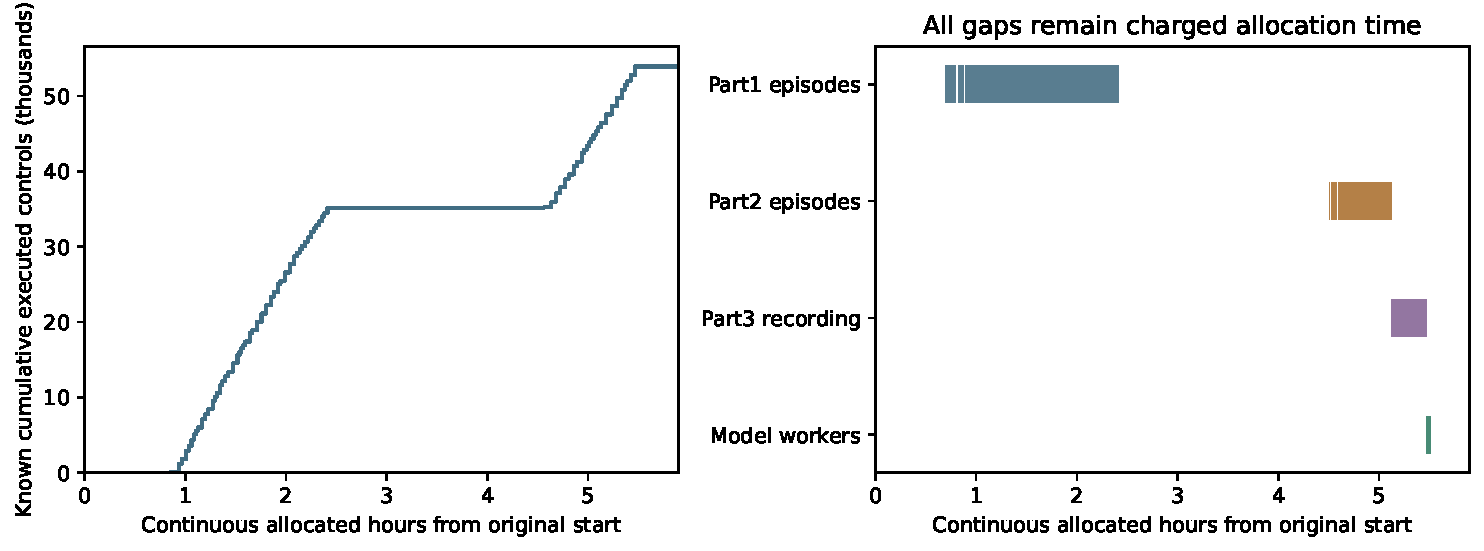
\includegraphics[width=.95\textwidth]{cumulative-costs.pdf}
\caption{Known controls and episode/model process intervals against the original
continuous allocation clock. Gaps include setup, implementation, reporting and idle
rental and remain charged. Model replay adds no physical experience. The graph is
an accounting snapshot, not a GPU-utilization estimate or rental-stop confirmation.}
\Description{Cumulative controls reach 53,911. Short physical/model runs occupy part
of a longer charged allocation; the clock never resets between studies.}
\label{fig:allocation}
\end{figure*}

New evidence contains 54 native camera clips, sixteen matched videos and 48 complete
full-episode camera strips. Every violation has before/at/after images, while other
episodes have start/middle/final images. The companion reports and complete gallery
are linked from the paper README. The 3.34 GB raw archive, including RGB and features,
is private and download/hash verified at dataset revision \texttt{a971f56192cd}.
The own trained artifacts are separately private and pinned at model revision
\texttt{e76969467146}; full revisions and file hashes are in the exports. Assets,
credentials and external checkpoints are excluded. Part 1's original episode
artifacts, protocol, lineage and adverse findings remain preserved.

\section{Interpretation and next decision}
The Part 1 training gain fails to transfer; Part 2 supplies no adaptive benefit
because its trigger never changes timing; Part 3 fails factual prediction accuracy
and correction-dependent calibration does not distinguish its proposed method from
ordinary disagreement. These are separate findings. Neither a timeout nor any one
case identifies a unique failure cause. The eight common data episodes and simple
forecast references supply direction while avoiding an unsupported physical ranking
experiment. No optimizer-superiority, calibrated-risk or safety-guarantee claim follows.

Part 4 retains a calibration low-risk miss but fails its separate development
warning trade-off and event support. It therefore supplies no acquisition,
diversity or repair comparison. The stronger visual-only ranking remains an
information-ablation lead with excessive false alarms at its frozen operating
point. Neither the absent development confident misses nor the unexecuted
search establishes that counterexample acquisition cannot work.

A later study should establish saved-input repeatability and useful trigger activation
on designated development data, validate prediction/readout generalization across
whole tasks, and require supported correction strata that make the proposed trust
rule distinct. The visual-only contrast motivates a readout information ablation.
These are hypotheses for a separately frozen study, not fixes demonstrated here.
Ordinary task-policy learning remains necessary for the broader contribution claim.

\begin{acks}
AI coding assistance was used for implementation, analysis code, prose and typesetting.
Experimental outcomes derive from the recorded simulator/monitor traces, and every
experimental picture is extracted from recorded native video or lossless captured RGB. The paper adapts the repository's
existing GECCO template without changing its archived experiment or results.
\end{acks}
\bibliographystyle{ACM-Reference-Format}
\bibliography{references}
\end{document}
